\subsection{Prototype \#1}
\label{sec:implementation:prototypes:prototype1}
The first prototype was an Android phone application, 
that showed the location of the user, 
the direction the phone was pointing, 
and the devices that were being pointed at.
The application used a $10 \times 10$ grid to simulate a square room, 
in which the user and the devices to be controlled were located.
A set of imaginary devices was hardcoded into the application with fixed positions, 
and the grid would look like the one shown in \Cref{table/prototype-grid}.
The user is positioned in the center at $(5,5)$ by default. 
This position can be changed by using the \texttt{Up}, \texttt{Down}, \texttt{Left} and \texttt{Right} buttons.
When the user's direction changes, 
a list of devices being pointed at is acquired, 
by calculating the angle between the user's position and the position of each device.
The direction is found using magnetic fields, 
such that \num{0} is north, \num{-90} is west, \num{90} is east, etc. 
The angle between each smart device and the user, 
is calculated finding the inverse tangent (arctangent), 
and then converting from radians to degrees (dividing \num{180} by $\pi$), 
such that we get:
\begin{equation}\label{eq:angle}
\var{angle} = 180 / \pi * \arctan(\var{user.y} - \var{device.y} / \var{user.x} - \var{device.x})
\end{equation}
where \var{user.x} and \var{user.y} are the $x$ and $y$ coordinates of the user and likewise for the device.
A screenshot of this application is shown in \Cref{fig:prototype1-app-screenshots}.

% Thalley: Måske lave om et et Tikz coordinatsystem i stedet for? Fylder unødvendigt meget imo. 
\begin{table}[!htb] 
    \centering
    \tiny
    \begin{TAB}(e){|c:c:c:c:c:c:c:c:c:c|}{|c:c:c:c:c:c:c:c:c:c|}
     &  &  &  &  &  &  &  &  & Stereo \\
     &  &  &  &  &  &  &  &  &  \\
     &  &  &  &  &  & \begin{tabular}[c]{@{}l@{}}Coffee\\ Maker\end{tabular} &  &  &  \\ 
     &  &  &  &  &  &  &  &  &  \\ 
    \begin{tabular}[c]{@{}l@{}}Garage\\ Door\end{tabular} &  &  &  &  &  &  &  &  &  \\ 
     &  & Lamp 2 &  &  &  &  &  &  &  \\
     &  &  &  &  &  &  &  &  &  \\ 
     &  &  &  &  &  &  &  &  &  \\ 
     &  &  &  &  &  &  &  &  &  \\ 
    Lamp 1 &  &  &  &  & TV &  &  &  &  \\
    \end{TAB}    
    \caption{Grid showing the position of devices. Lamp 1 is located at (0,0) and Stereo is located at (9,9)}
    \label{table/prototype-grid}
\end{table}

\begin{figure}[!htb]%
    \centering
    \subfloat{
        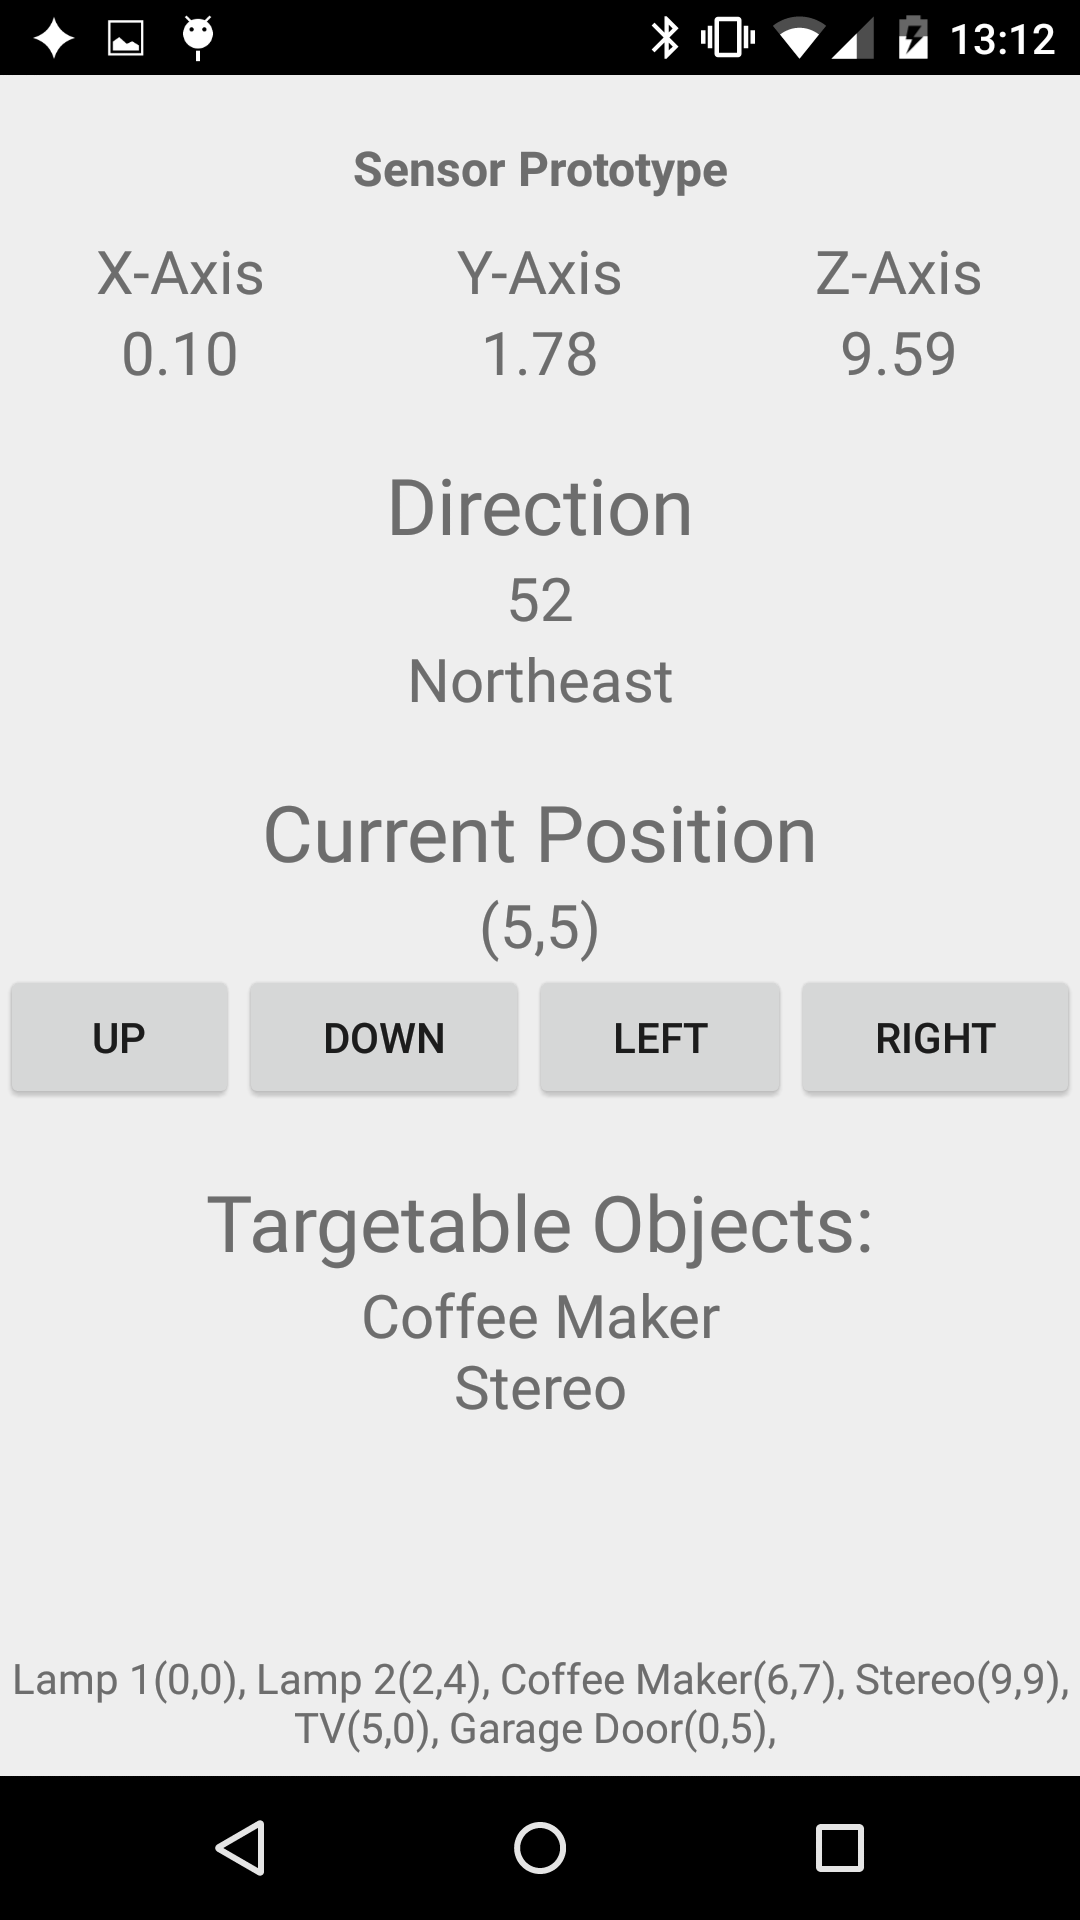
\includegraphics[width=0.3\textwidth]{images/Prototype1_Android_1.png}
    }
    \subfloat{
        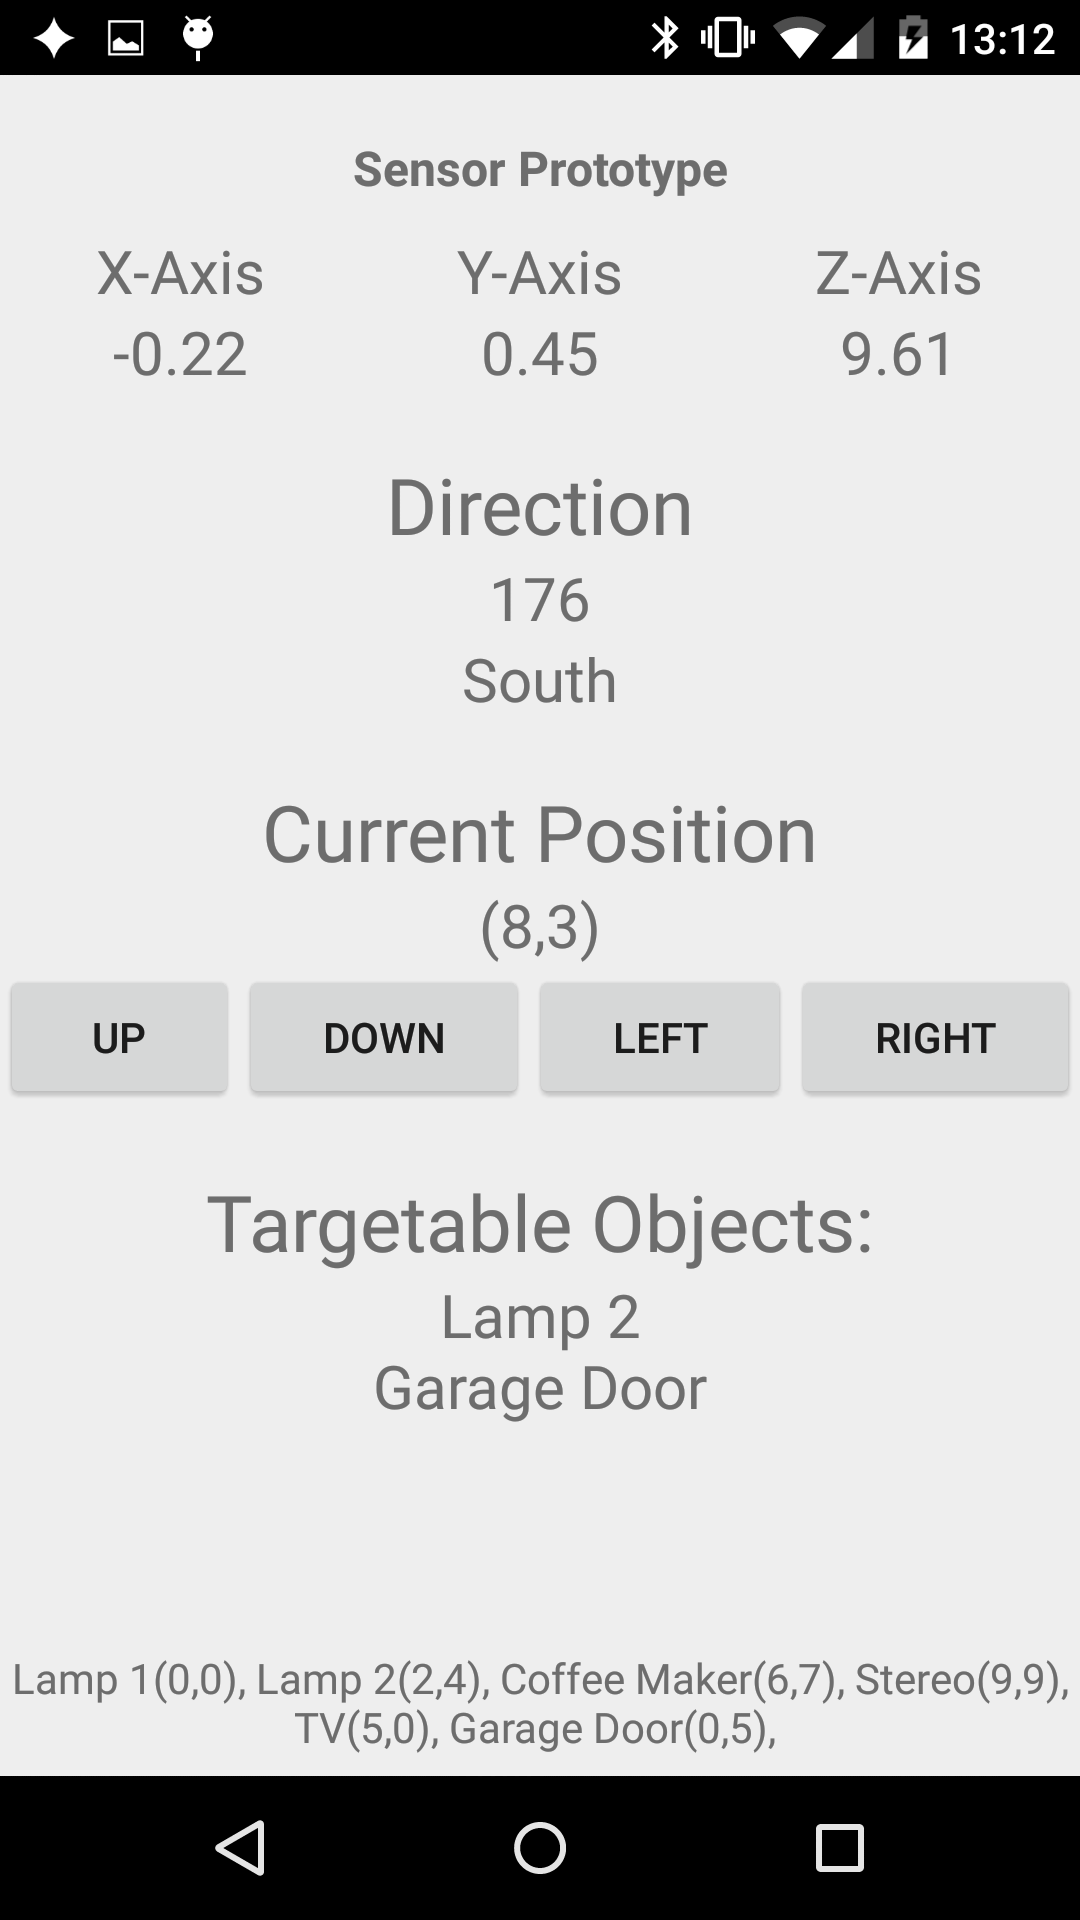
\includegraphics[width=0.3\textwidth]{images/Prototype1_Android_2.png}
    }
    \caption{Screenshots of the first prototype.}
    \label{fig:prototype1-app-screenshots}
\end{figure}

%%% Local Variables:
%%% mode: latex
%%% TeX-master: "../../master"
%%% End:
